\documentclass[11pt,a4paper]{article}
\usepackage[utf8]{inputenc}
\usepackage[T1]{fontenc}
\usepackage{lmodern}
\usepackage[margin=2.4cm]{geometry}
\usepackage{amsmath,amssymb}
\usepackage{graphicx}
\usepackage{booktabs}
\usepackage{xcolor}
\usepackage{hyperref}
\hypersetup{colorlinks=true,linkcolor=blue!50!black,urlcolor=blue!50!black}

\newcommand{\dd}{\mathrm{d}}
\newcommand{\kd}{k_1^{d}}

\title{Two springs in series, one of them damageable:\\
analytical, static and dynamic solutions}
\author{Repository \texttt{1D\_damage\_spring\_system}}
\date{\today}

\begin{document}
\maketitle

\section{Problem statement}

We consider two springs (elastic bars) in series:
\begin{center}
node 0 (clamped) $\;\xrightarrow{\;\text{spring 1, } \kd(u_1)\;}\;$ node 1 (mass $m_1$)
$\;\xrightarrow{\;\text{spring 2, } k_2\;}\;$ node 2 ($u_2$ imposed)
\end{center}
Spring 1 is damageable, spring 2 remains linear elastic. The loading is displacement
controlled: $u_2$ is imposed at node~2, increasing from $0$ to $u_2^f$. The unknown is the
displacement $u_1$ of the intermediate node. Spring 1 softens with damage, which produces a
\emph{snap-back}: the equilibrium branch $F(u_2)$ turns back in $u_2$, and quasi-static
displacement control cannot follow it. We compare:
\begin{enumerate}
  \item the \textbf{analytical} solution (closed form, complete branch including the unstable part);
  \item the \textbf{static} solution (Newton--Raphson at each $u_2$ increment);
  \item the \textbf{dynamic} solution (mass $m_1$ at node 1, implicit Newmark scheme,
        Newton--Raphson at each time step).
\end{enumerate}
The focus of the comparison is the shape of the residual $R(u_1)$ that the
Newton--Raphson has to cancel, and the way the inertia term regularises its non-monotonicity.

\subsection{Damage law}
The damage of spring 1 is a variable $d\in[0,1]$ depending on the maximum displacement reached
$\kappa = \max_{\tau\le t} u_1(\tau)$ (history variable, irreversibility):
\begin{equation}
  d(\kappa) = 1 - \exp\!\left(-\frac{\kappa^2}{u_c^2}\right),\qquad
  \kd(u_1) = k_1\,\bigl(1-d(\kappa)\bigr),\qquad
  F_1 = \kd\,u_1 .
\end{equation}
On loading ($u_1=\kappa$), $d'(u_1) = \dfrac{2u_1}{u_c^2}\exp(-u_1^2/u_c^2)$; on unloading
($u_1<\kappa$), $d$ is frozen and the spring unloads elastically with the secant stiffness
$k_1(1-d)$. For monotonic loading (analytical and static cases), $\kappa=u_1$ at all times.

\subsection{Parameters}
Consistent unit system N / mm / s, hence mass in tonne ($1\,\mathrm{t}=1000$~kg).
\begin{center}
\begin{tabular}{llr}
\toprule
Spring 1 & $E_1 = 10\,000$~MPa, $A_1 = 20$~mm$^2$, $L_1 = 5$~mm & $k_1 = E_1A_1/L_1 = 40\,000$~N/mm\\
         & $u_c = 5$~mm & \\
Spring 2 & $E_2 = 20\,000$~MPa, $A_2 = 30$~mm$^2$, $L_2 = 500$~mm & $k_2 = E_2A_2/L_2 = 1\,200$~N/mm\\
Mass     & $m_1 = 10$~t (node 1) & \\
Loading  & $u_2 : 0 \to u_2^f = 80$~mm & \\
Newton--Raphson & tolerance $|R|\le 10^{-6}$~N, 50 iterations max & \\
\bottomrule
\end{tabular}
\end{center}
The ratio $k_1/k_2 = 33.3$: spring 1 is very stiff while intact, and almost all of the
imposed displacement is absorbed by spring 2 ($u_1 \simeq u_2\,k_2/(k_1+k_2)$). The mass
$m_1=10$~t is not physical for a $20\,\mathrm{mm}^2\times5$~mm bar (actual mass
$\rho A_1 L_1\sim 10^{-6}$~t): it is a numerical regularisation parameter, see \S\ref{sec:dyn}.

\section{Analytical solution}
\label{sec:ana}
The equilibrium of node 1 reads
\begin{equation}
  R(u_1;u_2) = \kd(u_1)\,u_1 - k_2\,(u_2-u_1) = u_1\bigl(\kd(u_1)+k_2\bigr) - k_2u_2 = 0 .
  \label{eq:res}
\end{equation}
Rather than solving \eqref{eq:res} for $u_1$ at given $u_2$ (a transcendental equation with
several roots), we parametrise the equilibrium branch by $u_1$:
\begin{equation}
  u_2(u_1) = u_1\left(1+\frac{\kd(u_1)}{k_2}\right),\qquad
  F(u_1) = k_2\,(u_2-u_1) = \kd(u_1)\,u_1 = k_1\,u_1\,e^{-u_1^2/u_c^2}.
  \label{eq:ana}
\end{equation}
With $x=u_1/u_c$, the tangent stiffness of spring 1 is $\dd F/\dd u_1 = k_1 e^{-x^2}(1-2x^2)$ and
the system tangent is $k_t(u_1) = k_1e^{-x^2}(1-2x^2)+k_2$. Hence:
\begin{itemize}
  \item \textbf{force peak} at $x=1/\sqrt2$: $u_1 = u_c/\sqrt2 = 3.536$~mm,
        $F_{\max} = k_1 u_c e^{-1/2}/\sqrt2 = 85\,776$~N, $u_2 = 75.02$~mm;
  \item \textbf{limit point} (snap-back) where $\dd u_2/\dd u_1 = k_t/k_2 = 0$:
        $u_1 = 3.624$~mm, $u_2^{\lim} = 75.06$~mm; beyond it, $u_2$ decreases along the
        equilibrium branch down to $u_2 \simeq 13.3$~mm and then rises again on the fully
        damaged branch ($d\to1$, $F\to0$, $u_2\simeq u_1$).
\end{itemize}
Quasi-static displacement control therefore cannot go beyond $u_2^{\lim}$ without jumping, at
fixed $u_2$, from the state $(u_1 = 3.62,\;F=F_{\max})$ to the state $(u_1\simeq u_2,\;F\simeq0)$.

\paragraph{Energy balance of the jump.}
With the free energy $\Psi = \tfrac12 k_1(1-d)u_1^2 + \tfrac12 k_2(u_2-u_1)^2$ and the damage
dissipation $\mathcal D = \int Y\,\dd d$, $Y=\tfrac12 k_1u_1^2$, the work of the force along the
equilibrium branch between the two states of equal $u_2$ satisfies
$W = \int F\,\dd u_2 = \Psi_2-\Psi_1+\mathcal D_{\text{branch}}$. Since the jump occurs at
constant $u_2$ ($W=0$), the released energy is $\Psi_1-\Psi_2 = \mathcal D_{\text{branch}} + |W|$.
Numerically: $\Psi_1-\Psi_2 = 3\,217$~J, $\mathcal D_{\text{branch}} = 455$~J,
$|W| = 2\,762$~J. The area $|W|$ between the vertical jump and the equilibrium branch is thus
the energy released as kinetic energy at the jump, in excess of what the quasi-static branch
would have dissipated by damage. (The script calls it \texttt{released\_energy}.)

\section{Static solution}
\label{sec:stat}
$u_2$ is imposed over 2000 uniform increments and \eqref{eq:res} is solved by Newton--Raphson
with the analytical tangent
\begin{equation}
  k_t(u_1) = \kd(u_1) + u_1\,\frac{\dd\kd}{\dd u_1} + k_2,\qquad
  u_1^{(i+1)} = u_1^{(i)} - \frac{R(u_1^{(i)})}{k_t(u_1^{(i)})},
\end{equation}
starting from the solution of the previous increment. The residual \eqref{eq:res} is not
monotonic in $u_1$ ($k_t<0$ for $u_1\in[3.62\,;\,\simeq12]$~mm, minimum $k_t = -16\,650$~N/mm): at
a given $u_2$ it may have one or three roots (figure~\ref{fig:res}, left).

\paragraph{Handling of the jump.}
For $u_2 > u_2^{\lim}$ there is no longer a root in the neighbourhood of the previous iterate:
the Newton--Raphson cycles without converging (in the original scripts this case was not
detected and a non-converged value was stored). The solver now checks convergence and, on
failure, restarts the Newton--Raphson from the fully damaged branch ($u_1^{(0)}=u_2$): the
jump occurs at the first increment after the limit point ($u_2 = 75.08$~mm), consistently with
the analytical solution. Away from the jump, 4 iterations suffice.

\section{Dynamic solution}
\label{sec:dyn}
A mass $m_1$ is added at node 1; node 2 remains displacement controlled by a ramp
$u_2(t)=v_2\,t$ up to $u_2^f$, then held at $u_2^f$ for $n_{\text{hold}}$ steps to let the jump
complete. The equation of motion of node 1 (undamped) is
\begin{equation}
  m_1\ddot u_1 + \kd(u_1)\,u_1 - k_2\,(u_2(t)-u_1) = 0 .
\end{equation}

\paragraph{Newmark scheme.}
Implicit Newmark, $\beta=\tfrac14$, $\gamma=\tfrac12$ (average acceleration, unconditionally
stable, no numerical damping), in predictor--corrector form:
\begin{align}
  \tilde u &= u_n + \Delta t\,v_n + \tfrac{\Delta t^2}{2}(1-2\beta)\,a_n, &
  \tilde v &= v_n + (1-\gamma)\Delta t\,a_n,\\
  a_{n+1} &= c_1\,(u_{n+1}-\tilde u),\quad c_1 = \frac{1}{\beta\Delta t^2}, &
  v_{n+1} &= \tilde v + \gamma\Delta t\,a_{n+1}.
\end{align}
The residual to cancel at step $n+1$ and its tangent are those of the static case augmented
by the inertia term:
\begin{equation}
  R_{\text{dyn}}(u_1) = m_1c_1\,(u_1-\tilde u) + R(u_1;u_2^{n+1}),\qquad
  k_t^{\text{dyn}}(u_1) = m_1c_1 + k_t(u_1).
  \label{eq:resdyn}
\end{equation}
The Newton--Raphson is initialised with the predictor $\tilde u$. The history variable
$\kappa$ is frozen during the iterations of a step and updated after convergence.

\paragraph{Choice of the time step: inertial regularisation.}
From \eqref{eq:resdyn}, inertia adds to the tangent the constant $m_1c_1 = m_1/(\beta\Delta t^2)$.
If $m_1c_1 > -\min k_t = 16\,650$~N/mm, the dynamic residual is strictly increasing in $u_1$: a
single root, unambiguous Newton--Raphson, no more abrupt jump at the limit point. With the
natural pulsation of the intact system $\omega_0=\sqrt{(k_1+k_2)/m_1} = 64.2$~rad/s
($T_0 = 97.9$~ms) and $\Delta t = T_0/N$, the inertia/stiffness ratio is
\begin{equation}
  \frac{m_1c_1}{k_1+k_2} = \frac{N^2}{4\pi^2\beta} = \frac{N^2}{\pi^2}\quad(\beta=\tfrac14).
\end{equation}
A fine step ($N=40$, initial choice) gives a ratio $\simeq160$: the dynamic residual is an
almost perfect straight line and the comparison with statics loses its interest. We keep
$N=5$, i.e. $\Delta t = 19.6$~ms, $m_1c_1 = 104\,360$~N/mm, ratio $2.5$: enough to regularise
(minimum dynamic tangent $+87\,700$~N/mm) without flattening the contribution of the damaged
spring. The ramp lasts 150 steps ($2.94$~s, i.e. 30 natural periods: loading slow compared with
the system dynamics), followed by 100 hold steps. The Newton--Raphson converges in at most 3
iterations.

\paragraph{Results.}
The dynamic solution follows the analytical equilibrium branch beyond the limit point ($u_2$ up
to $\simeq78$~mm before $F$ drops, figure~\ref{fig:fu}), then node 1 ``jumps'' to the damaged
branch during the hold. Since the released energy (\S\ref{sec:ana}) has no dissipation
mechanism (no damping, spring 1 already fully damaged), the mass then oscillates freely on
spring 2 about $u_1 = u_2^f$ with period $2\pi\sqrt{m_1/k_2} = 0.574$~s and amplitude
$\simeq73$~mm (figure~\ref{fig:time}); $F_2$ then becomes alternately negative (spring 2 in
compression). Thanks to irreversibility ($\kappa$), damage stays at $d=1$ during these
oscillations; with the reversible law $d=d(u_1)$ of the original scripts, $d$ dropped back to
$0.66$ at the low point ($u_1\simeq5$~mm) and spring 1 ``healed'', which is non-physical.

\section{Figures}
\begin{figure}[h]\centering
  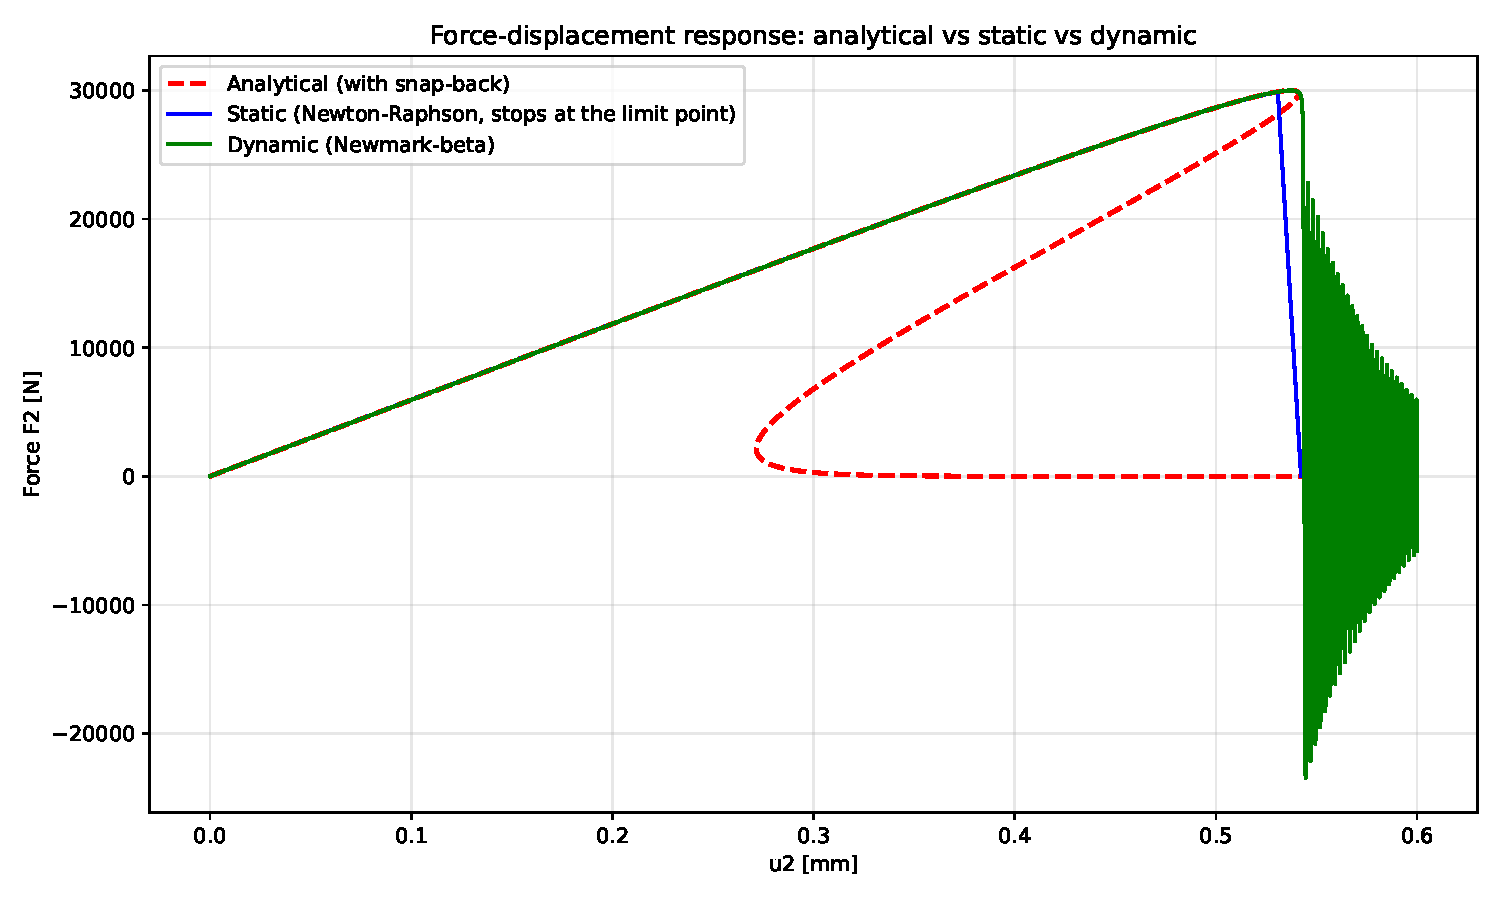
\includegraphics[width=.85\textwidth]{figures/force_displacement.pdf}
  \caption{Force--displacement response $F_2(u_2)$: analytical (complete branch with snap-back),
  static (jump at the limit point) and dynamic (passes the limit point, then jumps and oscillates).}
  \label{fig:fu}
\end{figure}
\begin{figure}[h]\centering
  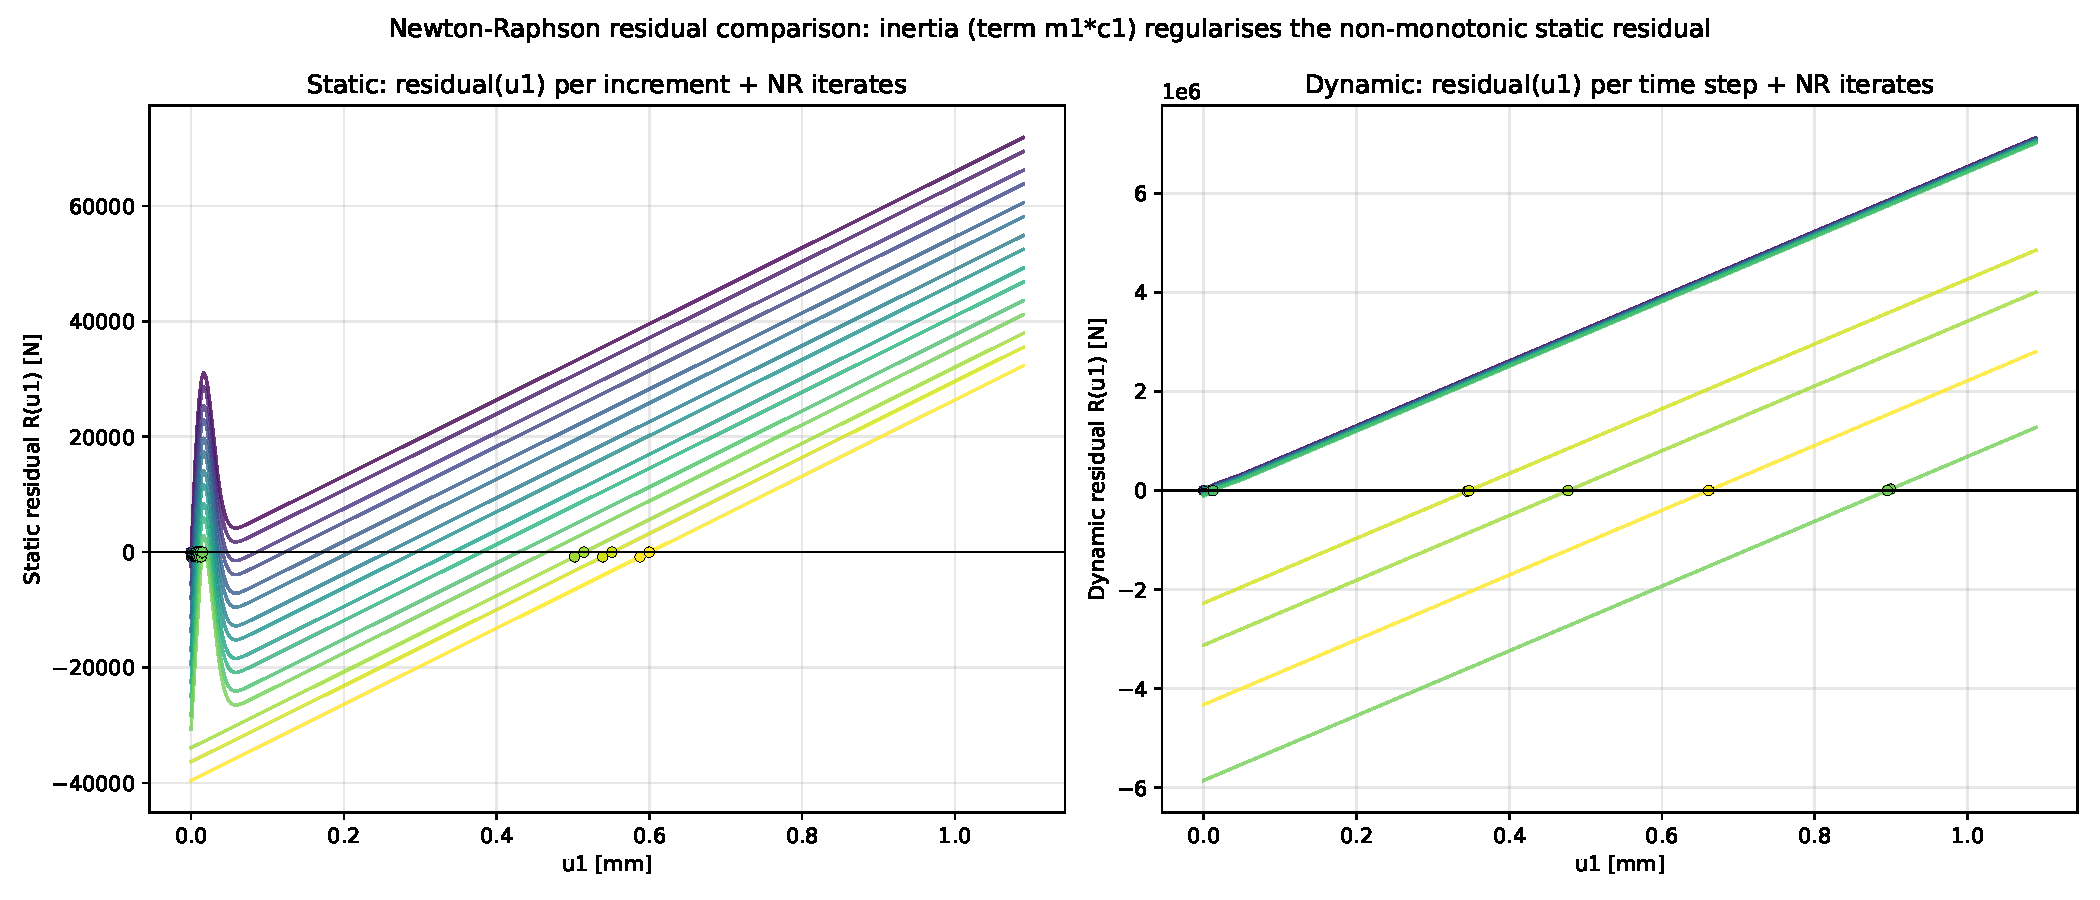
\includegraphics[width=\textwidth]{figures/residuals_static_dynamic.pdf}
  \caption{Residual $R(u_1)$ to be cancelled by the Newton--Raphson, one curve per increment
  (colour from purple, start of loading, to yellow, end) with the iterates as dots. Left: static,
  non-monotonic residual (bump due to the softening of spring 1), up to three roots. Right:
  dynamic, the term $m_1c_1(u_1-\tilde u)$ makes the residual strictly increasing; the curves
  shift vertically with $\tilde u$, which carries the kinematic history.}
  \label{fig:res}
\end{figure}
\begin{figure}[h]\centering
  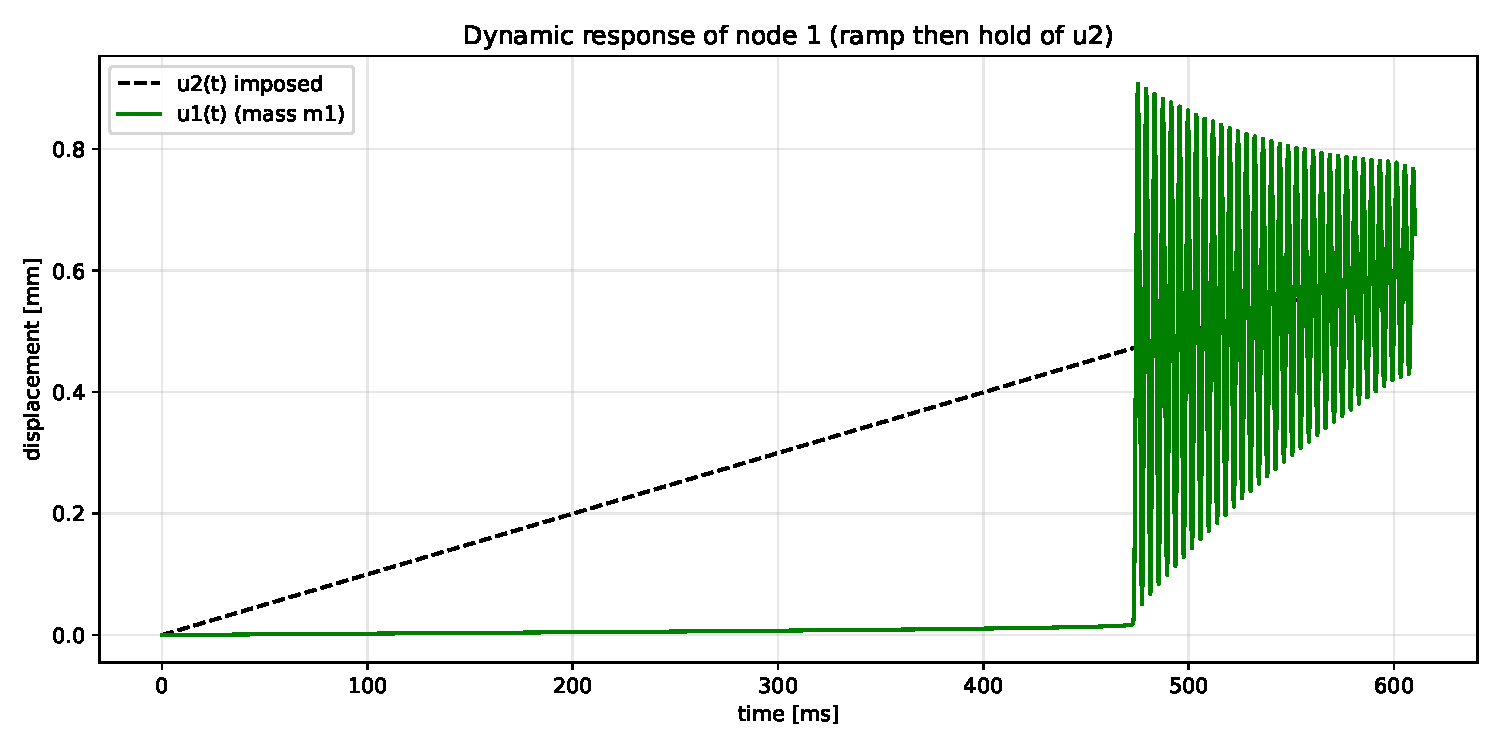
\includegraphics[width=.85\textwidth]{figures/time_response.pdf}
  \caption{Dynamic time response: ramp of $u_2$ then hold; jump of node 1 and undamped free
  oscillation on spring 2.}
  \label{fig:time}
\end{figure}

\clearpage
\section{Script layout and checks}
\begin{center}
\begin{tabular}{ll}
\toprule
\texttt{parameters.py} & physical and numerical parameters, derived quantities\\
\texttt{model.py} & damage law with $\kappa$, static residual/tangent, Newton--Raphson\\
\texttt{analytical\_solution.py} & branch \eqref{eq:ana}, peak, energy balance\\
\texttt{static\_solution.py} & $u_2$ increments, Newton--Raphson, restart at the jump, iterate history\\
\texttt{dynamic\_solution.py} & predictor--corrector Newmark, ramp + hold, iterate history\\
\texttt{comparison.py} & assembles the three solutions, figures (\texttt{--save} writes them to \texttt{figures/})\\
\bottomrule
\end{tabular}
\end{center}
Checks performed: numerical peak and limit point consistent with the analytical values;
identity $\Psi_1-\Psi_2 = \mathcal D_{\text{branch}}+|W|$ satisfied; Newton--Raphson convergence
at each increment/step (tolerance $10^{-6}$~N; a tolerance of $10^{-9}$~N was below the
round-off noise of the inertia terms $\sim10^7$~N); positivity of the dynamic tangent; period
of the free oscillations; conservation of $d=1$ after the jump.

\paragraph{Limitations and extensions.}
Non-physical mass (regularisation parameter); no damping, hence perpetual oscillations after
the jump (a damping $c\,\dot u_1$ or a dissipative Newmark $\gamma>\tfrac12$ would make them
decay); spring 2 is assumed massless; the restart at the static jump assumes that the other
stable branch is the fully damaged one, which is the case here.

\end{document}
